\newcommand{\tw}{\textwidth}
\newcommand{\vk}{\textbf{k}}
\documentclass[11pt]{article}

\usepackage{fullpage}
\usepackage{graphicx}
\usepackage{}
\usepackage{float}
\usepackage{caption}
\usepackage{subcaption}
\usepackage{amsmath}
\usepackage[spanish]{babel}

\pagestyle{empty}
\title{ Estructuras: C$_{16}$H$_{16}$--boat, \\ C$_{16}$H$_{8}$--up  y  C$_{16}$H$_{2}$ }
\date{}
%~~~~~~~~~~~~~~~~~~~~~~~~~~~~~~~~~~~~~~~~~ INICIO DEL DOCUMETO ~~~~~~~~~~~~~~~~~~~~~~~~~~~~~~~~~~~~~~~~~~~~~~~%
\begin{document}
\maketitle
\thispagestyle{empty}


\vspace{.5cm}

Te mando el reporte de c\'alculos para cada una de las estructuras en las que he estado trabajando con sus respectivas gr\'aficas e ilustraciones de la misma para identificarlas.

\section{Estructura C$_{16}$H$_{16}$--boat}

En la (fig. \ref{fig:boat}) se muestran dos vistas de la estructura C$_{16}$H$_{16}$--boat. Para esta estructura hice lo que me pediste para la respuesta lineal. Partiendo la ecuaci\'on de la respuesta lineal

\begin{equation}
	Im \left[ \chi^{ab}(\omega) \right] = \frac{\pi e^{2}}{\hbar} \int \frac{d \textbf{k}}{8 \pi^{3}} \sum_{vc} r^{a}_{vc}(\textbf{k}) r^{b}_{cv}(\textbf{k}) \ \delta (\omega_{cv}(\textbf{k}) -\omega) \label{eqn:lineal}
\end{equation}

la divid\'i para hacer dos casos de la misma, el primero conservando s\'olo $r^{a}_{vc}(\textbf{k})$ y despu\'es conservando \'unicamente $r^{b}_{cv}(\textbf{k})$ en el integrando. Para cada uno de los casos compil\'e e hice el c\'alculo de la respuesta usando s\'olo 10\,Ha como energ\'ia de corte. La gr\'afica correspondiente para distintas componentes y distinta cantidad de puntos \textbf{k} se muestra en la (fig. \ref{fig:lineal_boat}) 

\begin{figure}[h!]
	\begin{center}
		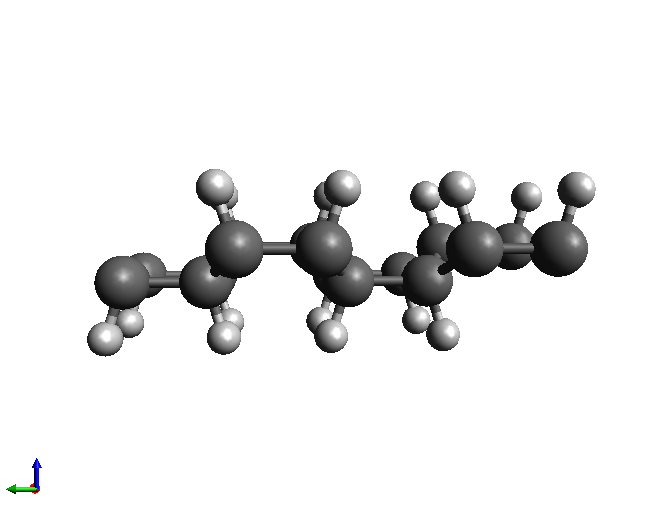
\includegraphics[width=0.45\textwidth]{./figures/boat/c16h16-boat-structure1}
		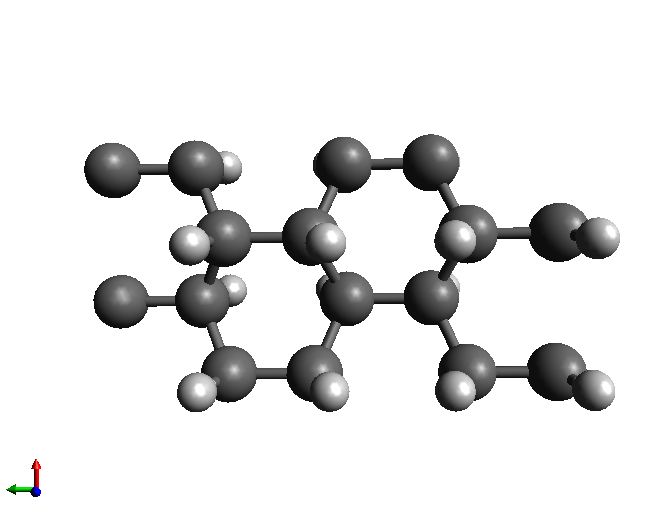
\includegraphics[width=0.45\textwidth]{./figures/boat/c16h16-boat-structure2}
	\end{center}
	\caption{Estructura C$_{16}$H$_{16}$--boat}
	\label{fig:boat}
\end{figure}

\begin{figure}
	\begin{center}
		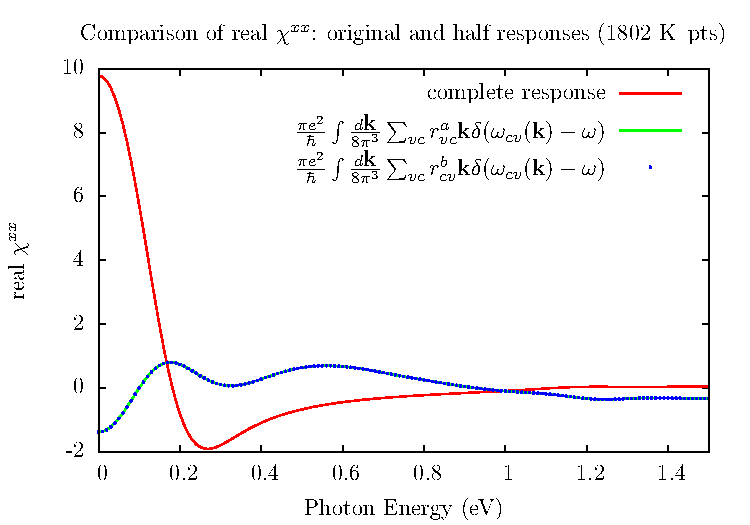
\includegraphics[width=0.65\textwidth]{./figures/boat/res1_chi_1_posMatElemen-1-2-original_sm}\\
		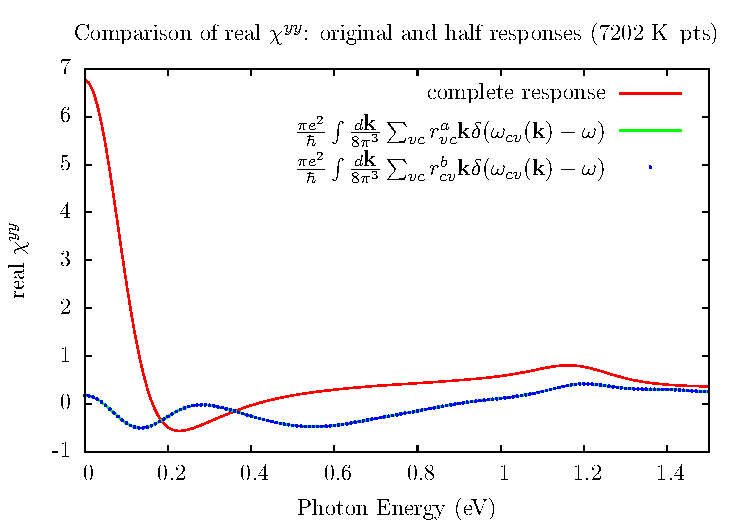
\includegraphics[width=0.65\textwidth]{./figures/boat/res1_chi_2_sposMatEleme-1-n-original2_m}\\
		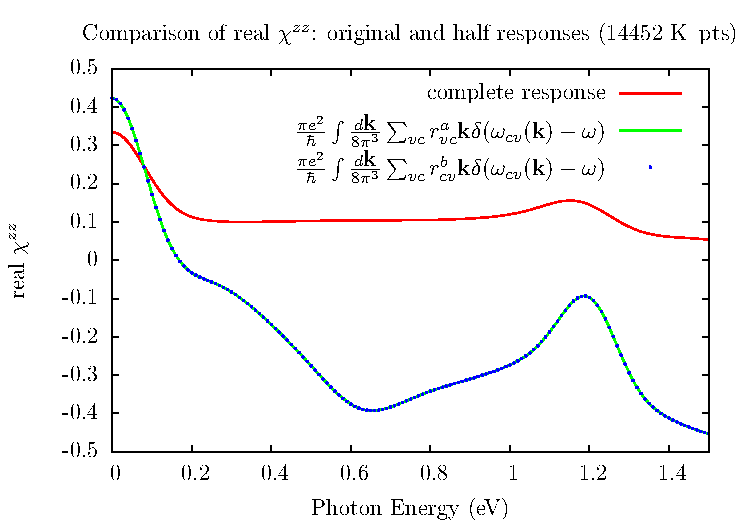
\includegraphics[width=0.65\textwidth]{./figures/boat/res1_chi_3_sposMatEleme-1-n-original2_m}
	\end{center}
	\caption{Respuesta lineal, completa e integrandos.}
	\label{fig:lineal_boat}
\end{figure}


\begin{figure}
	\begin{center}
		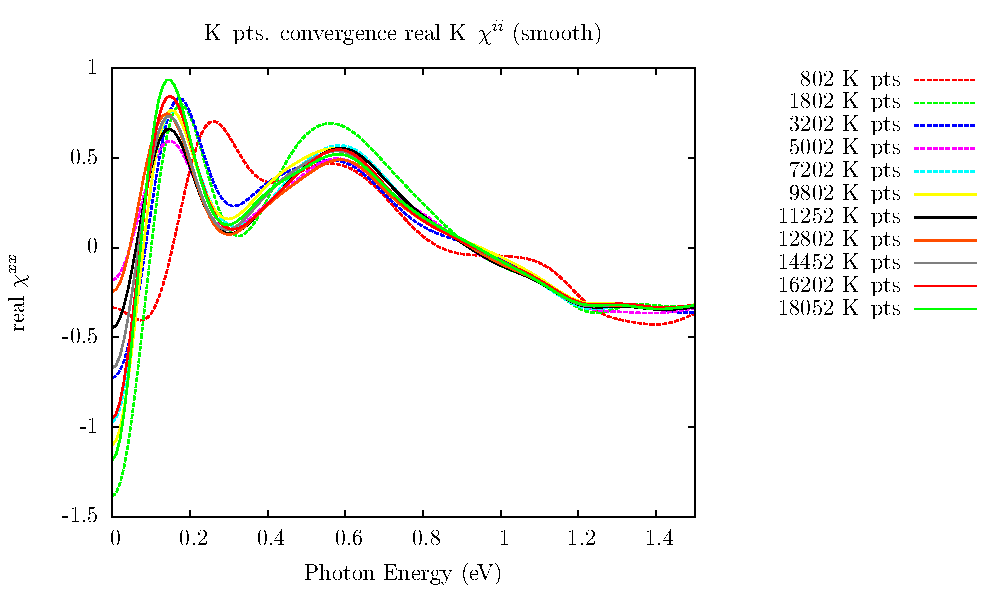
\includegraphics[width=0.65\textwidth]{./figures/boat/res1_chi_posMatElemen1_1_sm}\\
		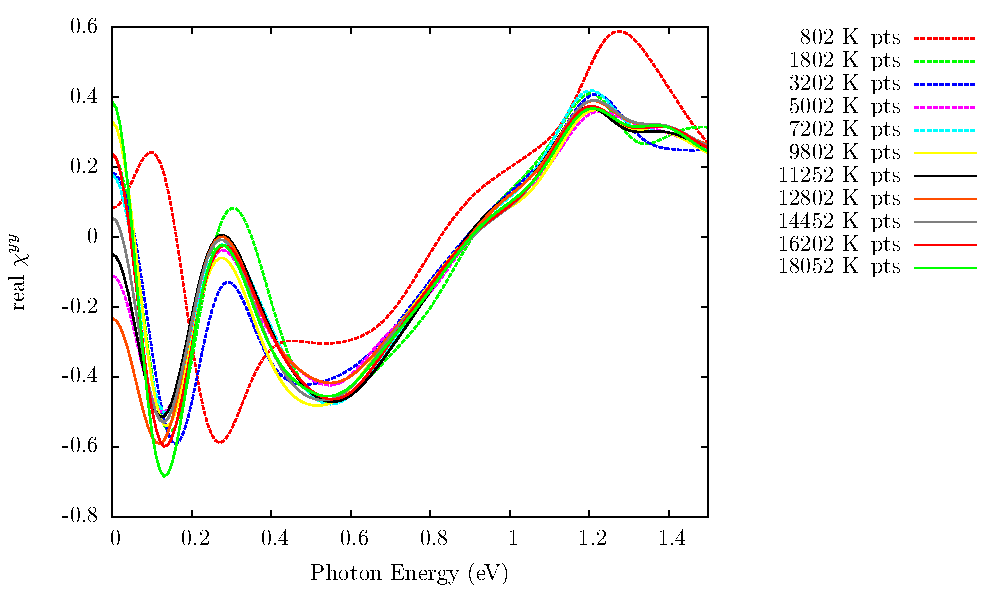
\includegraphics[width=0.65\textwidth]{./figures/boat/res1_chi_posMatElemen1_2_sm}\\
		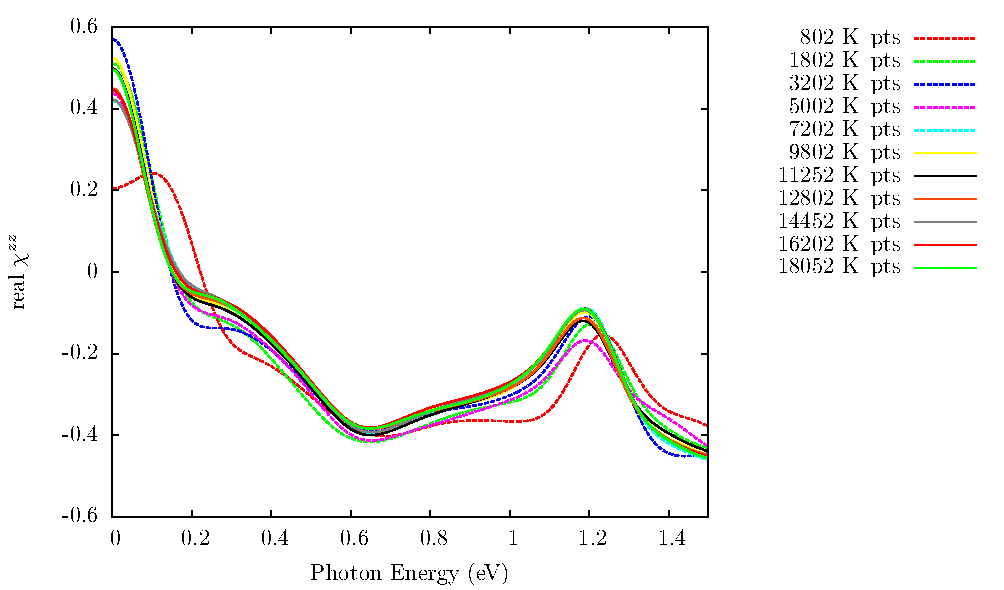
\includegraphics[width=0.65\textwidth]{./figures/boat/res1_chi_posMatElemen1_3_sm}
	\end{center}
	\caption{Respuesta lineal manteniendo s\'olo $r^{a}_{vc}(\textbf{k})$ en el integrando de la (Ec. \ref{eqn:lineal}). }
	\label{fig:lineal_posMatElemen1}
\end{figure}


Despu\'es de esto hice gr\'aficas para la convergencia para la respuesta lineal, manteniendo s\'olo la mitad del integrando. 

Puesto que la respuesta para cada una de las mitades es sim\'etrica \'unicamente incluyo, en la (fig. \ref{fig:lineal_posMatElemen1}), las respuestas manteniendo $r^{a}_{vc}(\textbf{k})$ en el integrando de la (Ec. \ref{eqn:lineal}). Como se puede ver, el comportamiento es similar al mostrado en la respuesta lineal completa que anteriormente te hab\'ia mandado.


\begin{figure}[h!]
	\begin{center}
		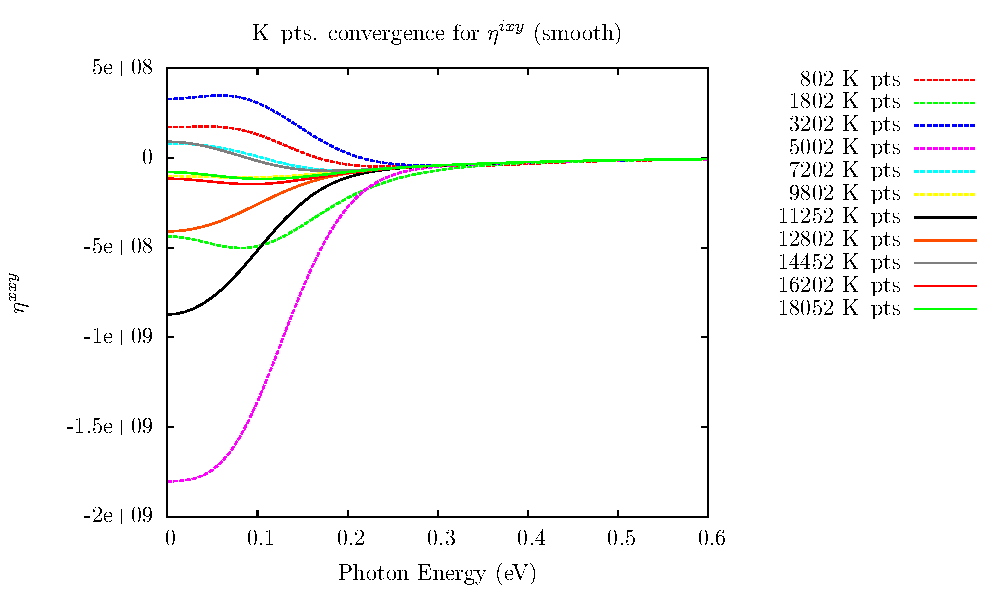
\includegraphics[width=0.9\textwidth]{./figures/boat/res3_eta_1_sm.pdf}
		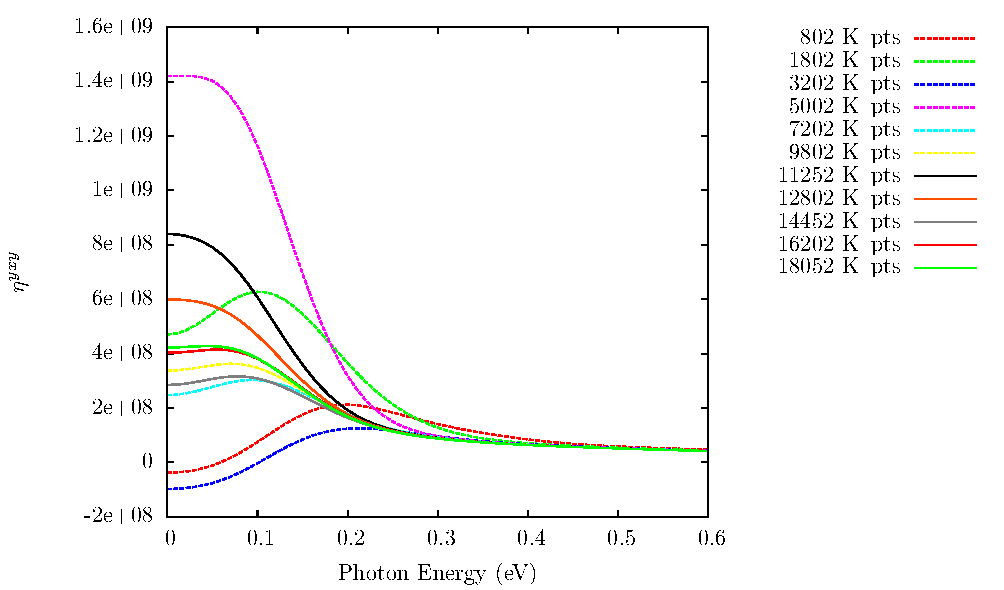
\includegraphics[width=0.9\textwidth]{./figures/boat/res3_eta_2_sm.pdf}
	\end{center}
\end{figure}

\begin{figure}[h!]
	\begin{center}
		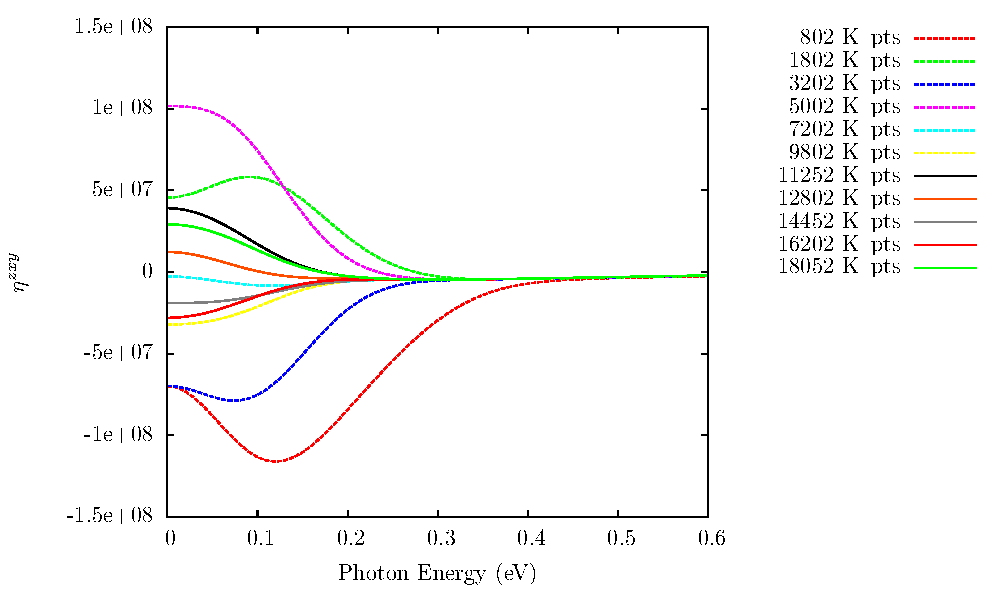
\includegraphics[width=0.9\textwidth]{./figures/boat/res3_eta_3_sm.pdf}
	\end{center}
	\caption{inyecci\'on de corriente, $\eta^{ixy}$, para distintos puntos \textbf{k}.}
	\label{fig:eta}
\end{figure}

En la (fig. \ref{fig:eta}) incluyo la respuesta a la inyecci\'on de corriente, $\eta^{ixy}$, para distintos puntos \textbf{k}. Al igual que como ha sucedido con otras respuestas para esta estructura, no hay convergencia.


Como tambi\'en ya te mencion\'e, una vez que acabe con lo que estoy corriendo, intentar\'e la convergencia utilizando la sintaxis que me mandaste para una red de puntos \textbf{k} desplazada. 


\section{Estructura C$_{16}$H$_{8}$--up}

En la (fig. \ref{fig:up}) se muestra la estructura C$_{16}$H$_{8}$--up. Esta es una de las dos estructuras trabajadas en la maestr\'ia. Como te mencion\'e en el correo, los c\'alculos anteriores son incorrectos. 

\begin{figure}[h!]
	\begin{center}
		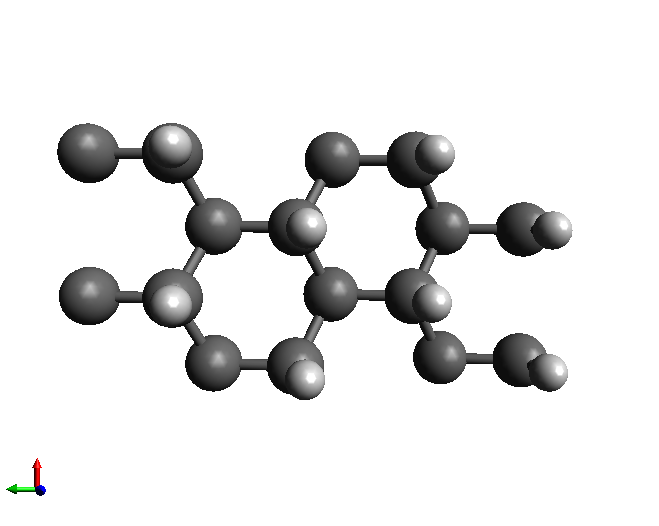
\includegraphics[width=0.45\textwidth]{./figures/up/c16h8_up-structure1}
		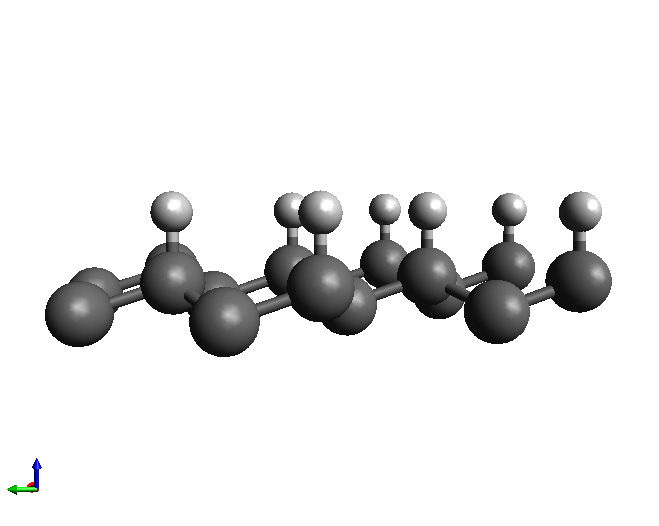
\includegraphics[width=0.45\textwidth]{./figures/up/c16h8_up-structure2}
	\end{center}
	\caption{estructura C$_{16}$H$_{8}$--up}
	\label{fig:up}
\end{figure}


\begin{figure}
	\begin{center}
		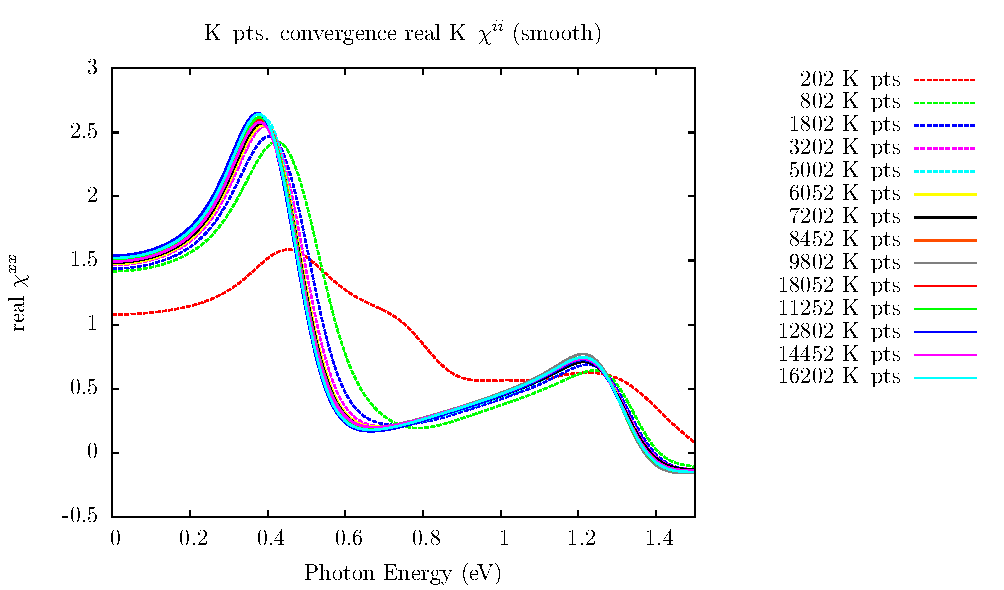
\includegraphics[width=0.75\textwidth]{./figures/up/res1_chi_1_sm.pdf}\\
		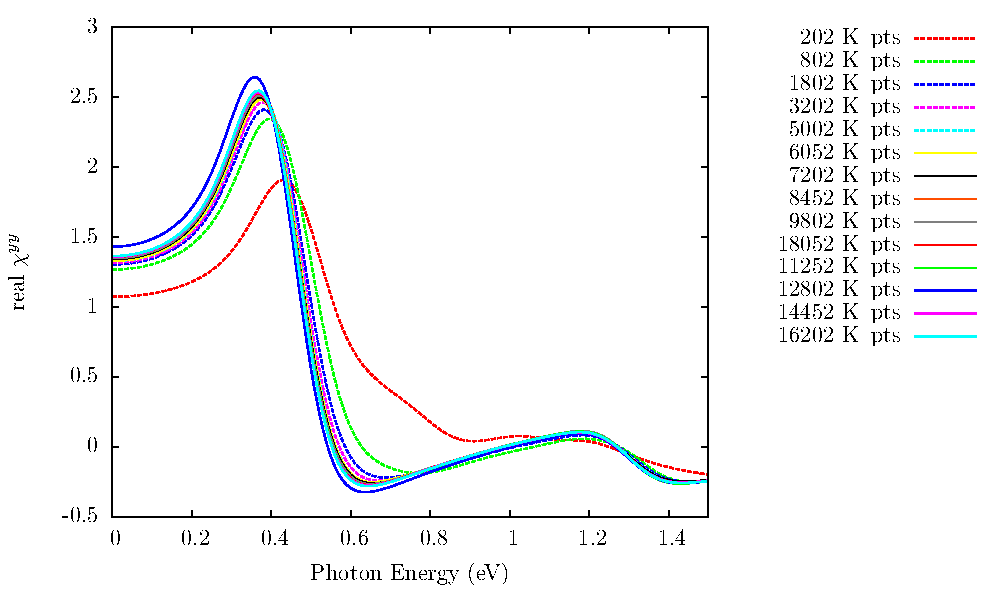
\includegraphics[width=0.75\textwidth]{./figures/up/res1_chi_2_sm.pdf}\\
		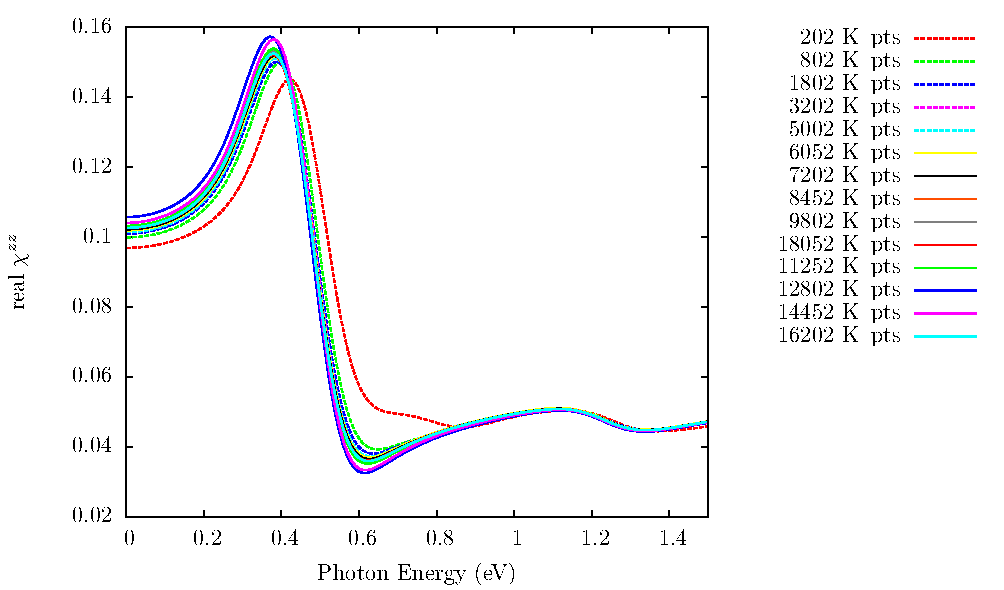
\includegraphics[width=0.75\textwidth]{./figures/up/res1_chi_3_sm.pdf}
	\end{center}
	\caption{Convergencia de puntos \textbf{k} para $\chi^{ii}$.}
	\label{fig:chi_up}
\end{figure}


\begin{figure}
	\begin{center}
		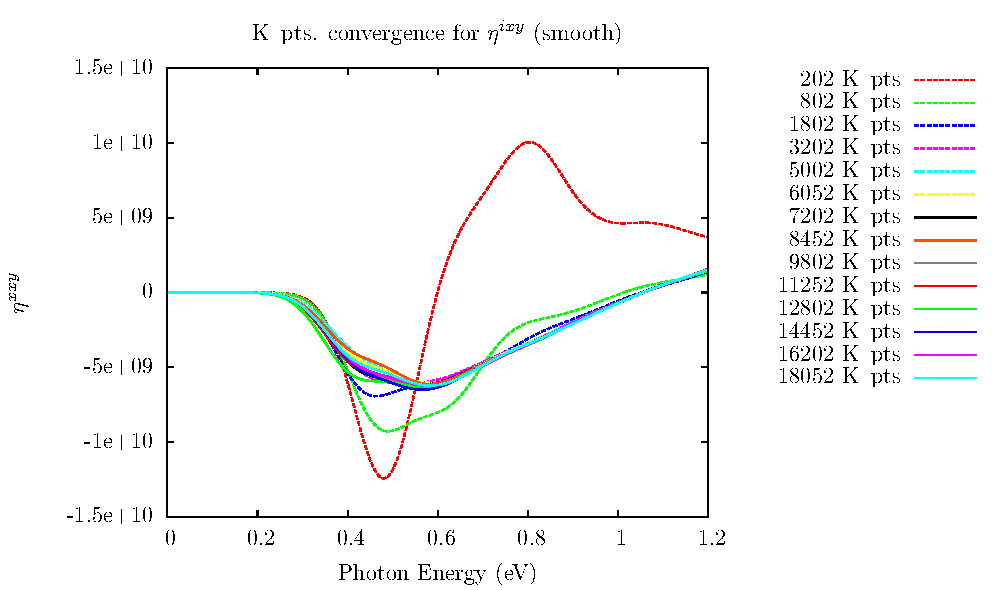
\includegraphics[width=0.75\textwidth]{./figures/up/res3_eta_1_sm.pdf}\\
		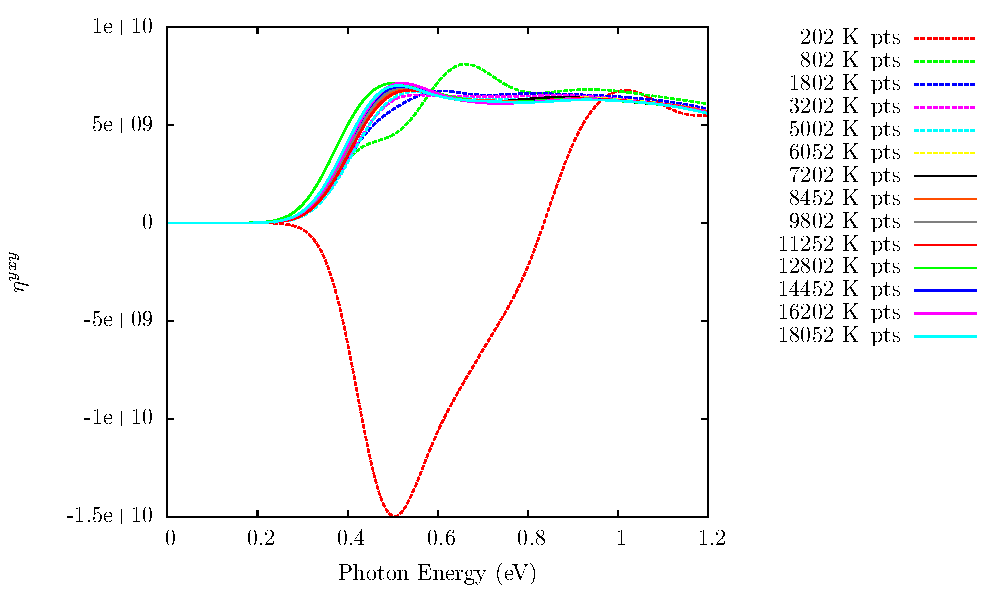
\includegraphics[width=0.75\textwidth]{./figures/up/res3_eta_2_sm.pdf}\\
		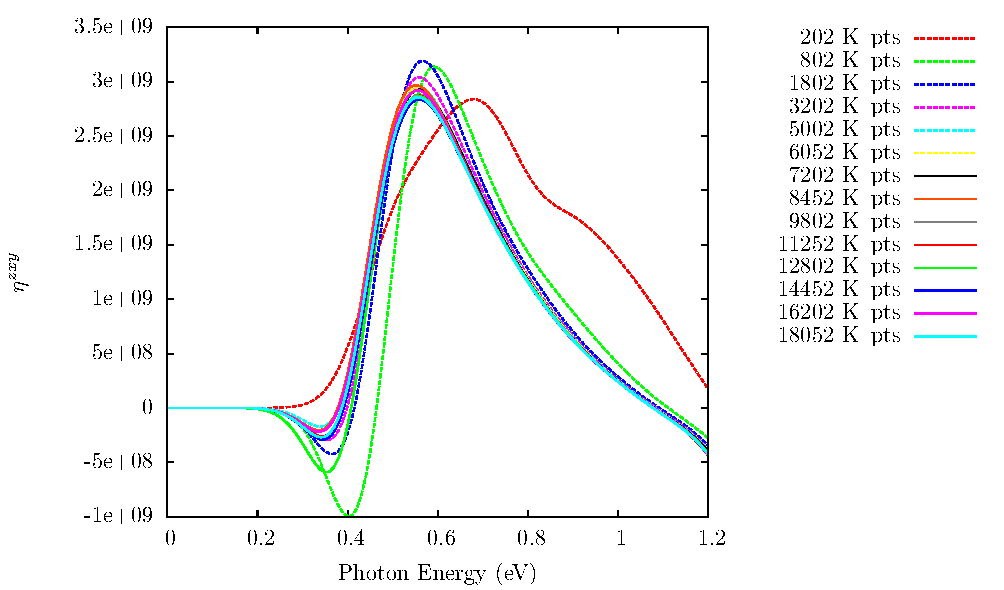
\includegraphics[width=0.75\textwidth]{./figures/up/res3_eta_3_sm.pdf}
	\end{center}
	\caption{Convergencia de puntos \textbf{k} para $\eta^{ixy}$.}
	\label{fig:eta_up}
\end{figure}


\begin{figure}
	\begin{center}
		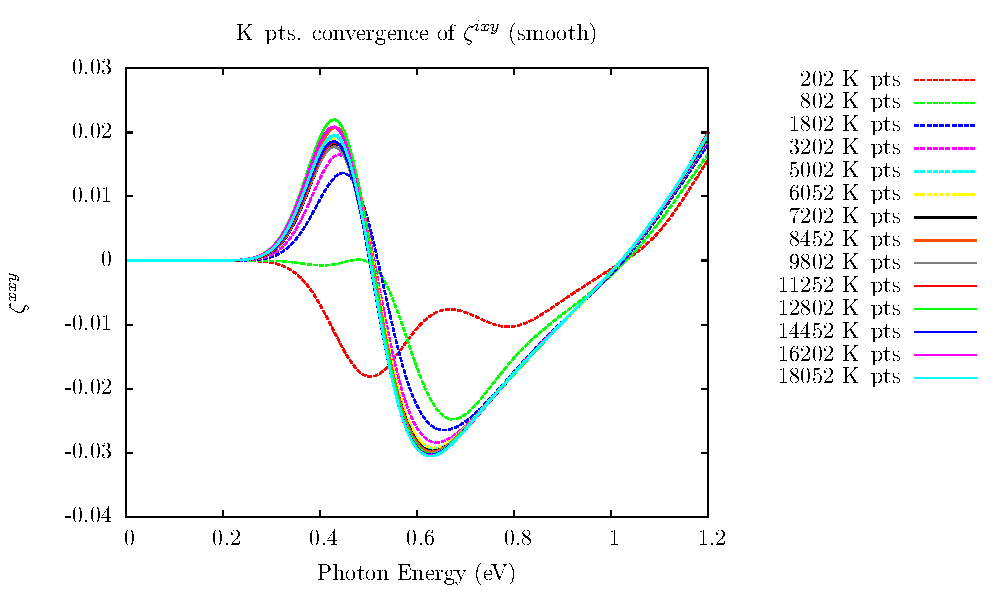
\includegraphics[width=0.75\textwidth]{./figures/up/res41_zeta_1_sm.pdf}\\
		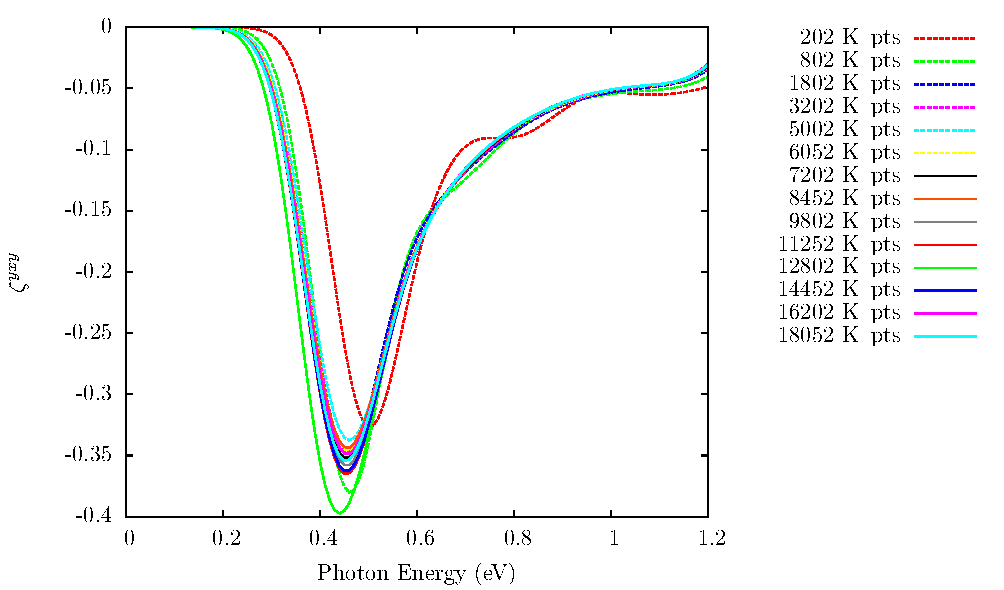
\includegraphics[width=0.75\textwidth]{./figures/up/res41_zeta_2_sm.pdf}\\
		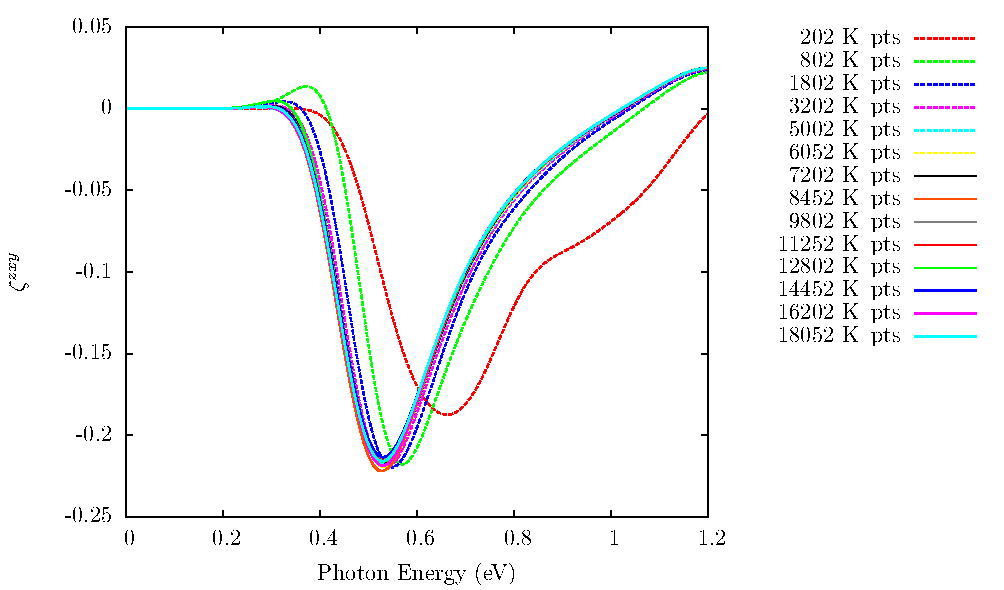
\includegraphics[width=0.75\textwidth]{./figures/up/res41_zeta_3_sm.pdf}
	\end{center}
	\caption{Convergencia de puntos \textbf{k} para $\zeta^{ixy}$.}
	\label{fig:zeta_up}
\end{figure}

\newpage

Para hacer la convergencia en puntos \textbf{k} utilic\'e como energ\'ia de corte 10\,Ha. Como se puede ver en las (figs. \ref{fig:chi_up}\,--\,\ref{fig:zeta_up}) hay convergencia en todas las respuestas para un valor de 6052 puntos \textbf{k} (salvo tu mejor observaci\'on).

En seguida comenzar\'e a hacer la convergencia para la energ\'ia de corte.

\section{Estructura C$_{16}$H$_{2}$}

Con esta estructura no se hab\'ia trabajado. Comenc\'e corriendo nuevamente con una energ\'ia de corte de 10\,Ha y 60 bandas como en los casos anteriores. Sucedi\'o que hab\'ia 66 bandas de valencia as\'i que tuve que revisar la convergencia para bandas de valencia.


\begin{figure}
	\begin{center}
		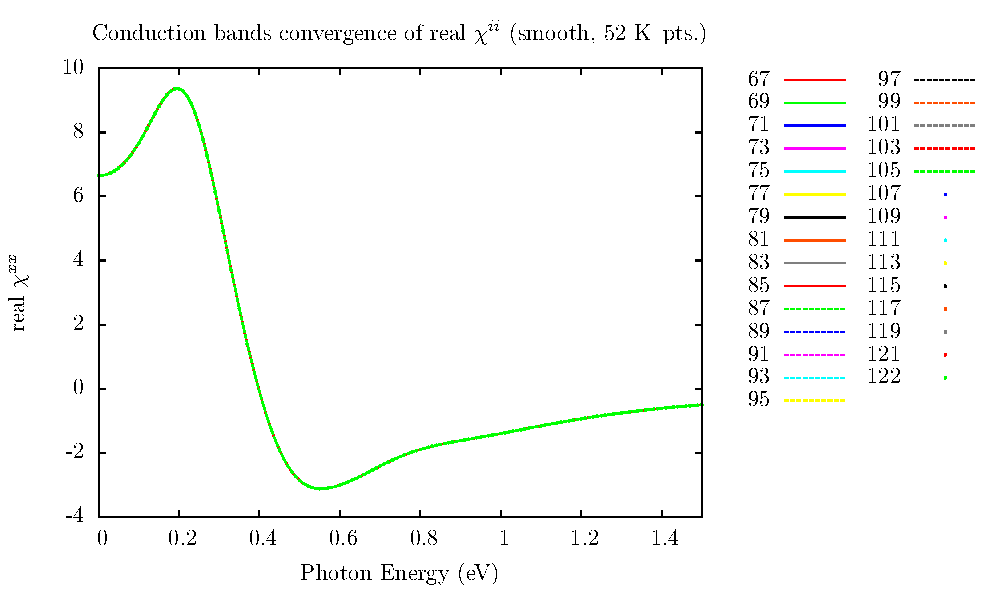
\includegraphics[width=0.75\textwidth]{./figures/12.5/res1_chi_1_sm_NCconv.pdf}\\
		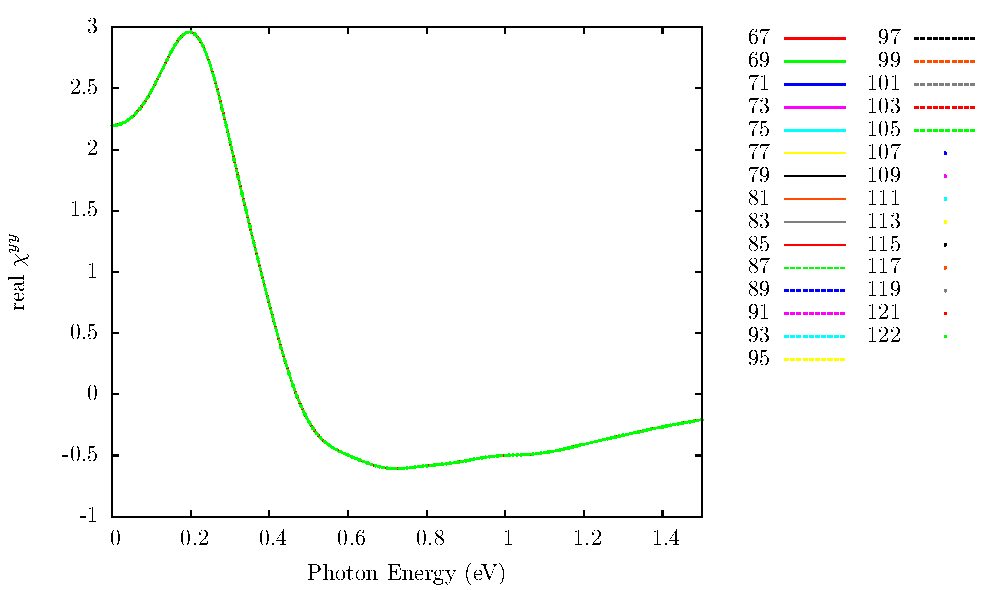
\includegraphics[width=0.75\textwidth]{./figures/12.5/res1_chi_2_sm_NCconv.pdf}\\
		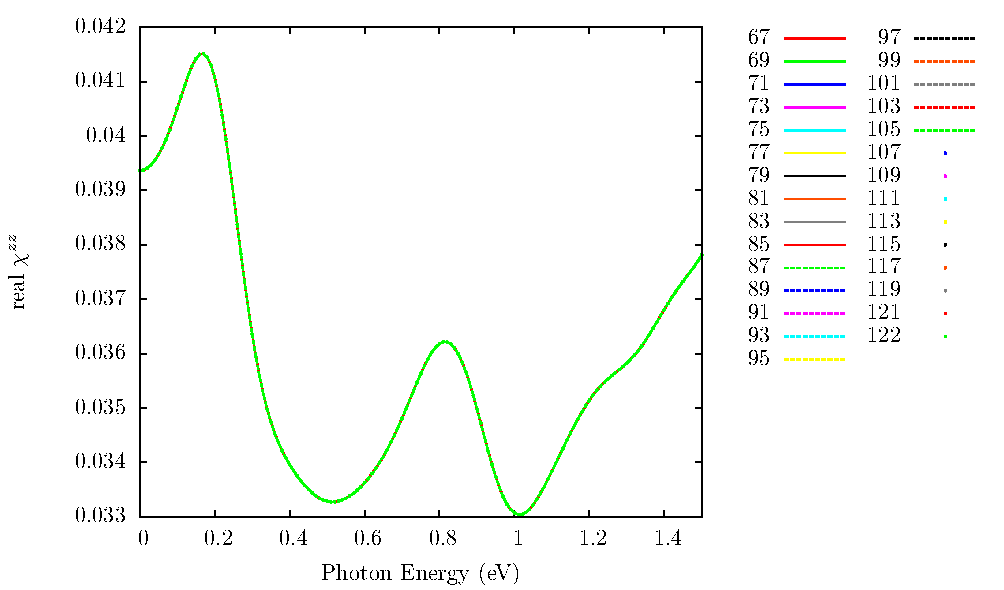
\includegraphics[width=0.75\textwidth]{./figures/12.5/res1_chi_3_sm_NCconv.pdf}
	\end{center}
	\caption{Convergencia en bandas de conducci\'on para $\chi^{ii}$.}
	\label{fig:chi_12.5}
\end{figure}

\begin{figure}
	\begin{center}
		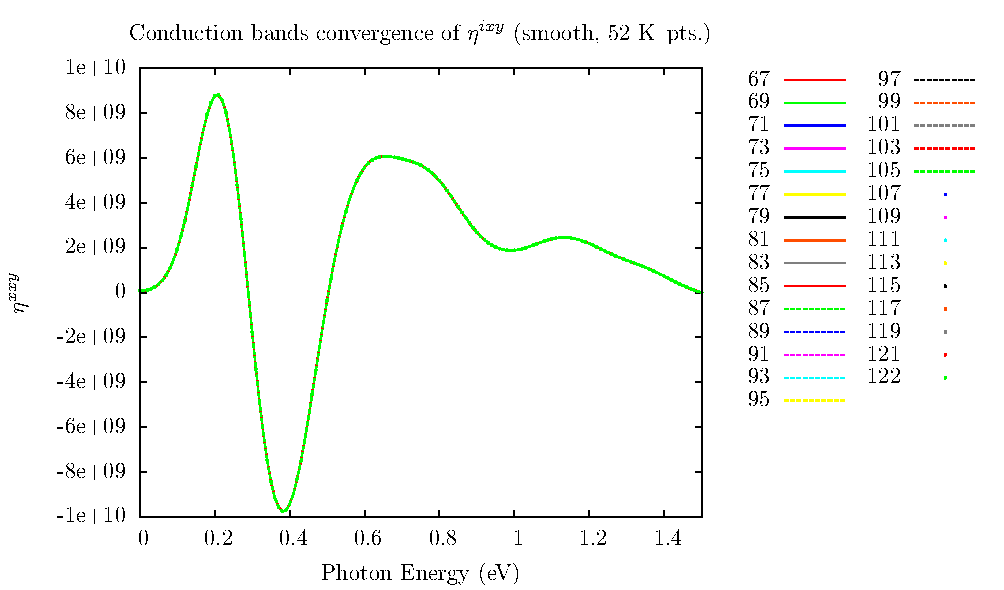
\includegraphics[width=0.75\textwidth]{./figures/12.5/res3_eta2_1_sm_NCconv.pdf}\\
		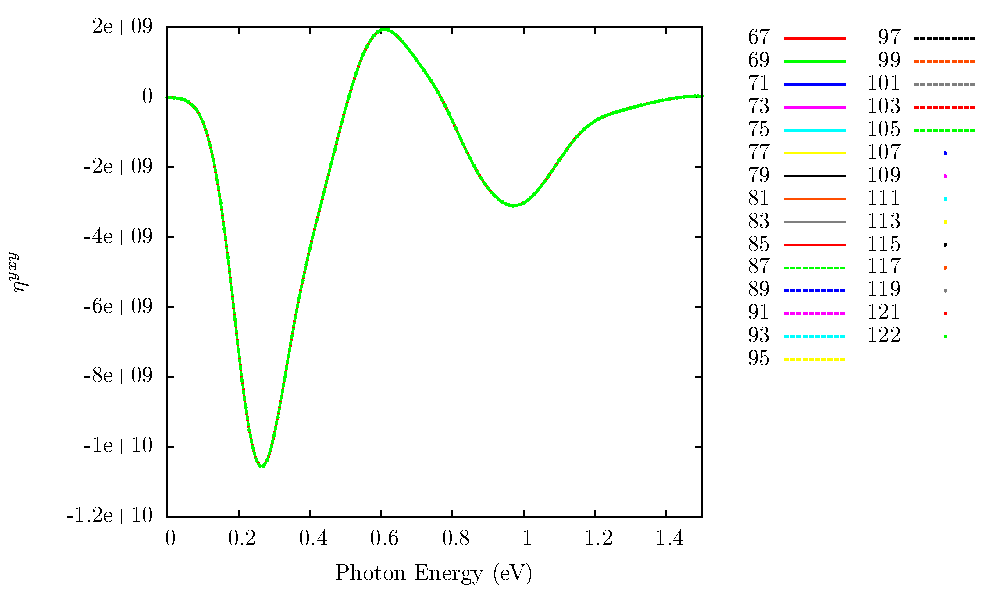
\includegraphics[width=0.75\textwidth]{./figures/12.5/res3_eta2_2_sm_NCconv.pdf}\\
		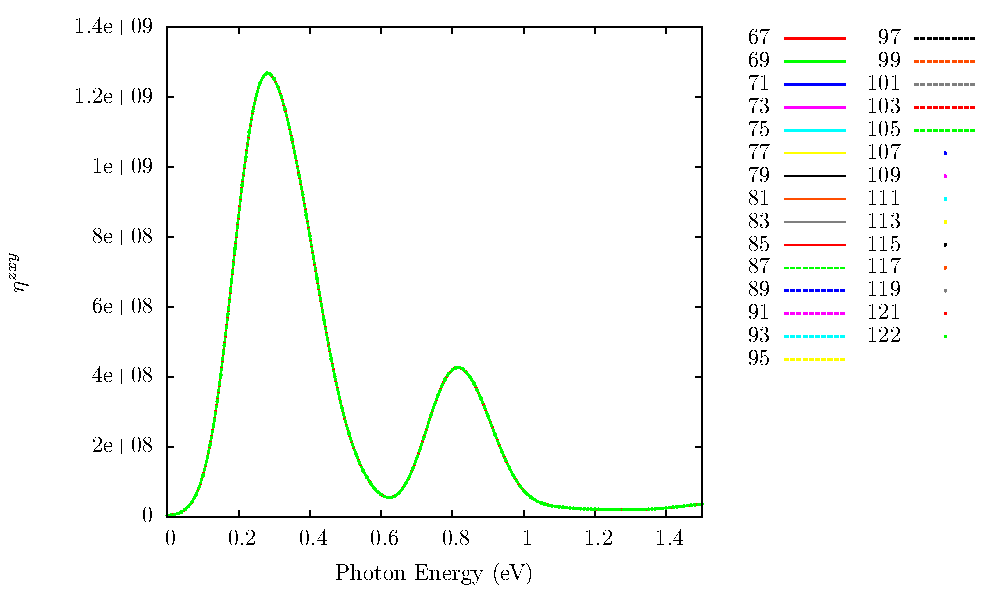
\includegraphics[width=0.75\textwidth]{./figures/12.5/res3_eta2_3_sm_NCconv.pdf}
	\end{center}
	\caption{Convergencia en bandas de conducci\'on para $\eta^{ixy}$.}
	\label{fig:eta_12.5}
\end{figure}
\begin{figure}
	\begin{center}
		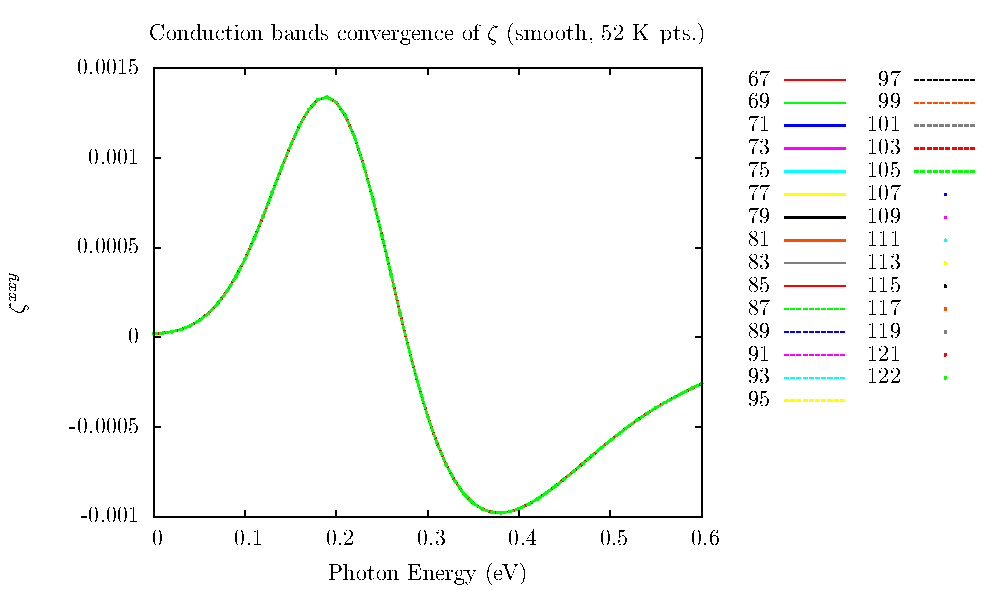
\includegraphics[width=0.75\textwidth]{./figures/12.5/res41_zeta_1_sm_NCconv.pdf}\\
		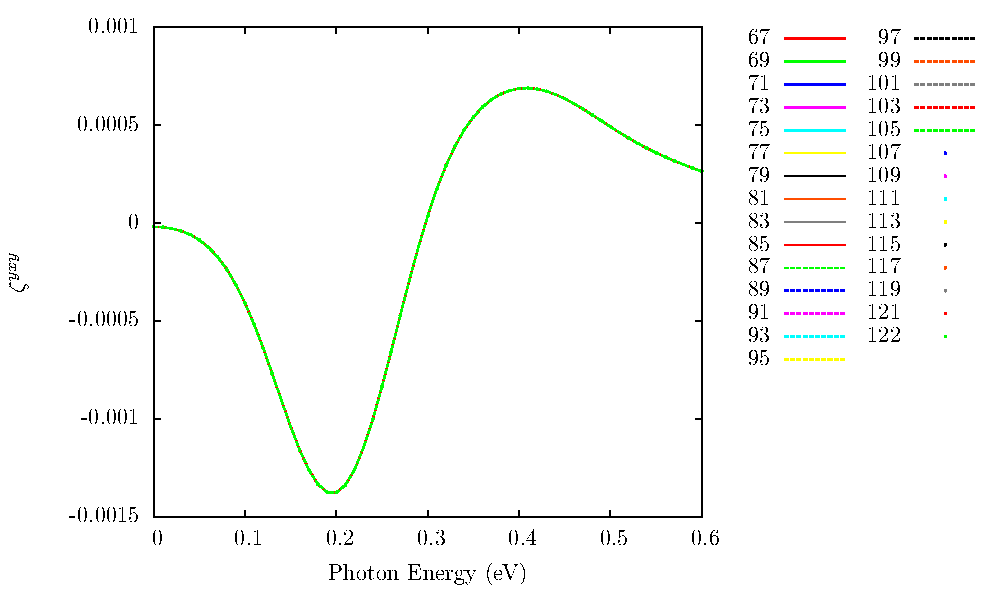
\includegraphics[width=0.75\textwidth]{./figures/12.5/res41_zeta_2_sm_NCconv.pdf}\\
		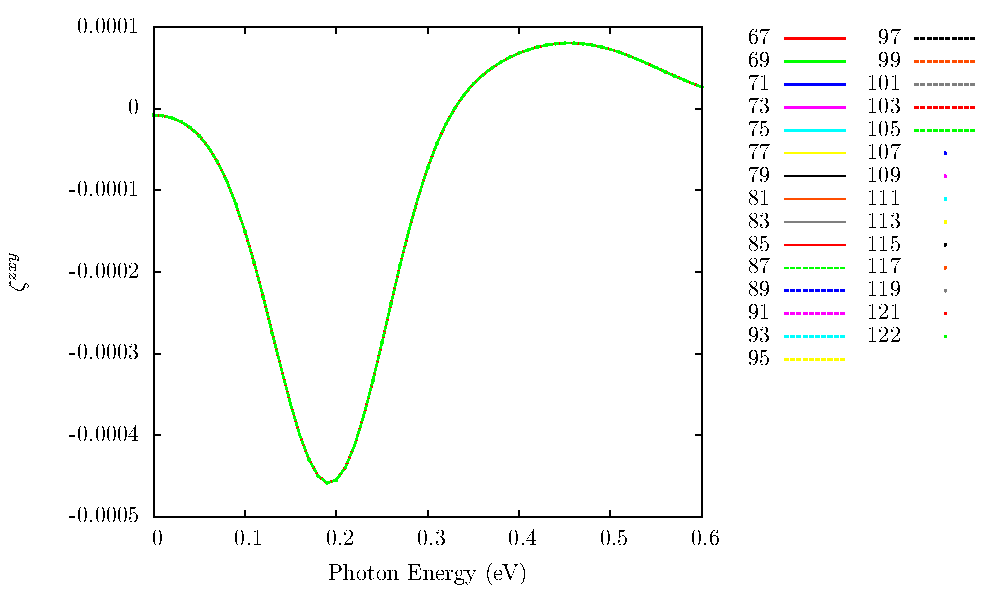
\includegraphics[width=0.75\textwidth]{./figures/12.5/res41_zeta_3_sm_NCconv.pdf}
	\end{center}
	\caption{Convergencia en bandas de conducci\'on para $\zeta^{ixy}$.}
	\label{fig:zeta_12.5}
\end{figure}

Para ello utilic\'e 122 bandas y s\'olo 52 puntos \textbf{k}. Como se puede ver en las (figs. \ref{fig:chi_12.5}\,--\,\ref{fig:zeta_12.5}). La convergencia para las bandas de valencia se da de inmediato. 

Actualmente estoy corriendo  convergencia para puntos \textbf{k} para esta estructura. Estoy usando 77 bandas para que el c\'alculo sea lo m\'as \'agil posible. En cuanto tenga los resultados de la convergencia de puntos para esta estructura te lo env\'io.

\end{document}

